% !TeX root = ../compleja.tex

\chapter{N\'umeros complejos y funciones}

\section{Operaciones aritm\'eticas en el cuerpo de los complejos}

En este curso estudiaremos el cuerpo $\C$ formado por el cuerpo de los números complejos.
\begin{dfn}[Número complejo. Parte real e imaginaria]
    Diremos que un número $z$ es \textbf{complejo} cuando sea una tupla de la forma $(a, b)$ (o equivalentemente $(a + bi)$) con $a, b \in \R$. Llamaremos parte real $\Re(z)$ y parte imaginaria $\Im(z)$ a cada escalar $a$ y $b$ de la tupla respectivamente.
\end{dfn}
\begin{dfn}[$\C$]
    Definimos $\C$ como el \textit{cuerpo} conformado por la estructura $\gen{\mtc C, +, \cdot}$, donde $\mtc C = \sdf{(a, b) \mid \forall a,b\ \in \R}$ y las operaciones $+$, $\cdot$ definidas como:
    $$
        (a, b) + (c, d) = (a + c, b + d)
    $$
    $$
        (a, b) \cdot (c, d) = (ac - bd, ad + bc)
    $$
\end{dfn}

\begin{pro}[$\C$ es un cuerpo]
    La estructura $\C = \gen{\mtc C, +, \cdot}$ definida anteriormente satisface las condiciones de ser un cuerpo.
\end{pro}
\begin{proof}
    Se deja al lector.
\end{proof}

\begin{eg}[C\'alculo de un inverso en $\C$]
    Por construcción el neutro de la suma en $\C$ es $(0, 0)$ y el de la multiplicación es $(1, 0)$. Vamos a buscar la expresión del inverso de un complejo $z = (a, b)$. Para ello buscamos resolver el sistema:
    $$
        (a, b) \cdot (x, y) = (1, 0)
    $$
    es decir:
    \begin{align*}
        ax - by &= 1\\
        -bx + ay &= 0
    \end{align*}
    que tiene solución cuando $a^2 + b^2 \neq 0$. Finalmente obtenemos:
    $$
        (x, y) = \left( \frac{a}{a^2+b^2}, \frac{-b}{a^2+b^2} \right)
    $$
    que como veremos más adelante implica que:
    $$
        z^{-1} = \frac{\cnj z}{\vabs{z}^2}
    $$
\end{eg}

Además, tiene sentido que si construimos $\C$ a partir de tuplas $\R\times \R$ entonces $\R \subseteq \C$. Nos interesa definir exactamente como, para ello establecemos la \textit{función de inclusión:} $\iota$\\
\fn{$\iota$}{$\R$}{$\C$}{$a$}{$(a, 0)$}

\begin{obs}
    En ocasiones usaremos indistintamente $(a, 0) \equiv a$ cuando un número complejo solo tenga parte real.
\end{obs}

Veremos más adelante que también podemos calcular las raíces de números complejos. En particular para las raíces cuadradas se reduce a resolver el sistema que se deduce de $(x, y)^2 = (a, b)$, es decir:
\begin{align*}
    x^2 - y^2 &= a\\
    2xy &= b
\end{align*}
que es un sistema resoluble, sin embargo la expresión no es nada agradable. Usaremos la \textit{representación polar} de los números complejos para simplificar esta tarea.

\subsection{Conjugaci\'on}
    \begin{dfn}[Conjugado de un número complejo]
        Definimos el \textbf{conjugado} de un número complejo $z = (a, b) \in \C$ como $\cnj z = (a, -b)$.
    \end{dfn}

    \begin{dfn}[Módulo de un número complejo]
        Definimos el \textbf{módulo} de un número complejo $z = (a, b) \in \C$ como $\rho = \vabs{z} = \sqrt{a^2 + b^2} \in \R$.
    \end{dfn}

    \begin{pro}[Propiedades del conjugado de un número complejo]
        Sea $z = (a, b) \in \C$:\\
        \begin{enumerate}[(1)]
            \item $z \cdot \cnj z = (a^2 + b^2) = \vabs{z}^2$
            \item $\cnj{z \cdot w} = \cnj z \cdot \cnj w$
            \item $\cnj{z + w} = \cnj z + \cnj w$
            \item $\cnj{\cnj z} = z$
            \item $z + \cnj z = 2 \cdot \Re(z)$
            \item $z - \cnj z = 2 \cdot \Im(z)$
            \item $z = \cnj z \iff z \in \R$
            \item Si $w \neq 0$, $\cnj{\frac{z}{w}} = \frac{\cnj z}{\cnj w}$
        \end{enumerate}
    \end{pro}
    \begin{proof} Consideraremos $z = (a, b)$ y $w = (c, d)$.
        \begin{enumerate}
            \item $$(a, b) \cdot (a, -b) = (a \cdot a - b \cdot(-b), a \cdot (-b) + b \cdot a) = (a^2 + b^2, 0)$$
            \item
            \begin{align*}
                \cnj{z\cdot w} &= \cnj{(ac - bd, ad + bc)} = (ac - bd, -ad -bc) =\\
                &= (ac - (-b) (-d), a(-d) + c(-b)) = (a, -b) \cdot (c, -d) = \cnj z \cdot \cnj w
            \end{align*}
            \item $$
                \cnj{z + w} = \cnj{(a + c, b + d)} = (a + c, -b -d) = (a, -b) + (c, -d) = \cnj z + \cnj w
                $$
            \item $$\cnj{\cnj{z}} = \cnj{(a, -b)} = (a, b) = z$$
            \item $$z + \cnj z = (a, b) + (a, - b) = (2a, 0) = 2 \Re(z)$$
            \item $$z - \cnj z = (a, b) - (a, - b) = (0, 2b) = 2 \Im(z)$$
            \item $$ z = \cnj z \iff a = a \text{ y } b = -b \iff b = 0 \iff z \in \R$$
            \item Vamos a demostrar primero que $\cnj{\frac{1}{w}} = \frac{1}{\cnj w}$:
            $$
                1 = w \cdot \frac{1}{w} \implies 1 = \cnj 1 = \cnj{w \cdot \frac{1}{w}} = \cnj{w} \cdot \cnj{\frac{1}{w}}
            $$
            y como $\C$ es un cuerpo sabemos que $\cnj{w}^{-1}$ existe, por tanto, multiplicando a ambos lados por $\cnj{w}^{-1}$ obtenemos:
            $$
                \frac{1}{\cnj{w}} = \cnj{\frac{1}{w}}
            $$
            Con este resultado ya es directo demostrar que:
            $$
                \cnj{\frac{z}{w}} = \cnj z \cdot \cnj{\frac{1}{w}} = \cnj z \frac{1}{\cnj w} = \frac{\cnj z}{\cnj w}
            $$
        \end{enumerate}
    \end{proof}
\subsection{Desigualdad triangular}
    En esta sección vamos a ver algunas propiedades de los números complejos así como la desigualdad triangular y su generalización.
    \begin{pro}[Propiedades del módulo de un número complejo]
        De nuevo consideramos $z = (a, b)$, $w = (c, d)\in \C$, $\sdf{z_i=(a_i, b_i)}_{i\in \N} \subset \C$.
        \begin{enumerate}
            \item $\vabs{z \cdot w} = \vabs{z} \cdot \vabs{w}$.
            \item $\vabs{z} = \vabs{-z} = \vabs{\cnj z} = \vabs{-\cnj z}$.
            \item $\vabs{\Re(z)} \leq \vabs{z}$ y $\vabs{\Im(z)} \leq \vabs{z}$.
            \item $\vabs{z + w} \leq \vabs{z} + \vabs{w}$. (Desigualdad triangular).
            \item $\vabs{z} - \vabs{w} \leq \vabs{z + w}$.
            \item $\vabs{ \vabs{z} - \vabs{w} } \leq \vabs{z + w}$.
            \item $\vabs{z_1 + \cdots + z_n} \leq \vabs{z_1} + \cdots + \vabs{z_n}$. (Desigualdad triangular generalizada).
        \end{enumerate}
    \end{pro}
    \begin{proof} En la gran mayoría de apartados se procede a demostrar la relación de los cuadrados, ya que al ser $f(x) = \sqrt{x}$ una función estrictamente creciente para números positivos, basta tomar raíces a ambos lados y llegamos a relación original.
        \begin{enumerate}
            \item $$\vabs{z \cdot w}^2 = (ac-bd)^2+(ad+bc)^2 = a^2c^2 \cancel{-2abcd} + b^2d^2 + a^2d^2 +\cancel{2abcd} + b^2c^2 = (a^2+b^2)(c^2+d^2) = \vabs{z}^2 + \vabs{w}^2$$
            \item Los cuatro términos se pueden abreviar en $\tilde z = (\pm a, \pm b)$ y entonces: $$\vabs{\tilde z} = \sqrt{(\pm a)^2 + (\pm b)^2} = \sqrt{a^2 + b^2} = \vabs{z}$$
            \item Como $\vabs{z}^2 = \vabs{\Re(z)}^2 + \vabs{\Im(z)}^2$ entonces es claro que:
            $$
                \vabs{\Re(z)}^2 \leq \vabs{\Re(z)}^2 + \vabs{\Im(z)}^2 \text{ y } \vabs{\Im(z)}^2 \leq \vabs{\Re(z)}^2 + \vabs{\Im(z)}^2
            $$
            \item
            \begin{align*}
                \vabs{z + w} &\leq \vabs{z} + \vabs{w}\\
                \vabs{z + w}^2 &\leq (\vabs{z} + \vabs{w})^2\\
                (z+w)\cnj{(z+w)} &\leq \vabs{z^2} + \vabs{w^2} + 2\vabs{z}\vabs{w}\\
                (z+w)(\cnj z + \cnj w) &\leq \vabs{z^2} + \vabs{w^2} + 2\vabs{z}\vabs{w}\\
                \vabs{z^2} + \vabs{w^2} + z\cnj w + \cnj z w &\leq \vabs{z^2} + \vabs{w^2} + 2\vabs{z}\vabs{w}\\
                \cancel 2\cdot\Re(z\cnj w) = z \cnj w + w \cnj z &\leq \cancel 2 \vabs{z} \vabs{w}\\
                \Re(z\cnj w) &\leq \vabs{z}\vabs{w} = \vabs{z}\vabs{\cnj w} = \vabs{z\cnj w}
            \end{align*}
            \item
            $$
                \vabs{z} = \vabs{z + w - w} \leq \vabs{z + w} + \vabs{-w} = \vabs{z + w} + \vabs{w} \implies \vabs{z} - \vabs{w} \leq \vabs{z + w}
            $$
            Análogamente demostramos la segunda desigualdad expresando $\vabs{w} = \vabs{w + z - z}$.
            \item Directa de la propiedad anterior y la desigualdad triangular.
            \item Por inducción sobre el número de términos del sumatorio de la desigualdad triangular. Sabemos que el caso base se cumple ($n=2$), ahora suponemos que se cumple para $n$ sumandos y lo probamos cierto para $n+1$, es decir, suponemos que es cierto:
            $$
                \vabs{\sum_{i=1}^{i=n} z_i} \leq \sum_{i=1}^{i=n} \vabs{z_i}
            $$ y entonces:
            $$
                \vabs{\sum_{i=1}^{i=n+1} z_i} = \vabs{z_{n+1} + \sum_{i=1}^{i=n} z_i} \leq \vabs{z_{n+1}} + \vabs{\sum_{i=1}^{i=n} z_i} \leq \vabs{z_{n+1}} + \sum_{i=1}^{i=n} \vabs{z_i} = \sum_{i=1}^{i=n+1} \vabs{z_i}
            $$
        \end{enumerate}
    \end{proof}
\subsection{Representaci\'on polar}
    Los números complejos, al estar construidos como un par ordenado de números reales se pueden representar geométricamente en el plano complejo (similar a $\R^2$). De esta forma, el número $z = a + bi = (a, b)$ se puede representar como el punto $(a, b)$ de $\R^2$.\\\\
    Además, toman especial importancia los puntos de la circunferencia unidad, (los que satisfacen la ecuación $x^2 + y^2 = 1$). Usando un poco de trigonometría podemos obtener fácilmente que los puntos del plano complejo que se corresponden con los de la circunferencia unidad son $(\cos \theta, \sin \theta)$.

    \begin{obs}
        Los números complejos no tienen una expresión única en esta forma ya que $(\cos \theta, \sin \theta) = (\cos (\theta + 2k\pi), \sin  (\theta + 2k\pi) )$ con $k \in \Z$.\\
        El $(0, 0)$ no tendría sentido expresarlo de forma polar, lo denominaremos simplemente $0$.
    \end{obs}

    \begin{center}
        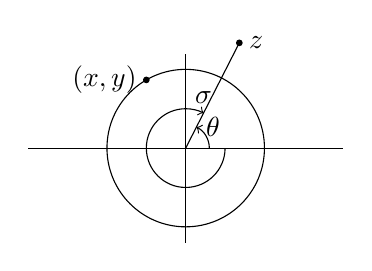
\begin{tikzpicture}
            \path (63: 1.5) coordinate (P);
            \path (120:1) coordinate (Q);
            \path (0: 0.3) coordinate (R);
            \path (0: 0.5) coordinate (R1);
            \draw (0, 0) ellipse (1cm and 1cm);
            \draw (-2, 0) -- (2, 0);
            \draw (0, -1.2) -- (0, 1.2);
            \filldraw[black] (P) circle (1pt) node[anchor=west] {$z$};
            \filldraw[black] (Q) circle (1pt) node[anchor=east] {$(x, y)$};
            \draw (0, 0) -- (P);
            \draw[->] (R) arc (0:63:0.3) node[anchor=west] {$\theta$};
            \draw[->] (R1) arc (360:63:0.5) node [anchor=south] {$\sigma$};
        \end{tikzpicture}
    \end{center}

    De esta forma, cualquier número complejo $z$ podrá expresarse como $z = \vabs{z}(\cos \theta, \sin \theta)$. Usualmente denominaremos a $\theta$ como el argumento de $z$, es decir, $\theta=\arg(z)$. Además, es común encontrar el módulo expresado con la letra $\rho$. Con esto podremos expresar $z$ como:\\
    $$
        z = \rho(\cos \theta, \sin \theta) = \rho(\cos \theta + i \sin \theta)
    $$

    Cuando definamos la exponencial compleja veremos que podemos expresar $z$ de la forma $z = \rho e^{i\theta}$.

    \begin{obs} %%TODO: Referenciar la imagen
        Como se aprecia en la figura superior, el argumento de $z$ no es único, tanto $\sigma$ como $\theta$ son el argumento de z (debido a que $\sigma = \theta - 2\pi$).\\

        Debido a que $\arg(z)$ es una función multievaluada (si $\arg(z) = \theta \implies \arg(z) = \sdf{\theta + 2n \pi \mid n \in \Z}$), en ocasiones querremos usar una función que escoja un solo argumento de ellos. La denominamos \textbf{argumento principal} ($\Arg{z}$), y la definimos restringiendo la imagen de $\arg{z}$ al intervalo $\left[0, 2\pi\right)$ o $\left[-\pi, pi\right)$.\\

        Sin embargo, aun habiendo determinado un argumento principal, en ninguno de los dos casos la función $\Arg()$ es continua en todo punto. Se puede ver que no existe una determinación continua del argumento.
    \end{obs}

    Esta forma de representar los números complejos nos simplificará varias tareas, como multiplicarlos o hallar raíces.
%%%%%%%%%%%%%%%%%%%%%%%%%%%%%%%%%%%%%%%%%%%%%%%%%%%%%%%%%%%%%%%%%%%%%%%%%% 30/01

    \begin{obs}
        Sea $\rho(\cos \theta, \sin \theta) = z = a + bi \implies \frac{b}{a} = \tan{\theta}$. Esto no significa que $\theta = \tan^{-1}\left(\frac{b}{a}\right)$ ya que la imagen de $\tan^{-1} \subseteq \left(-\frac{\pi}{2}, \frac{\pi}{2}\right)$.
    \end{obs}

    En general, encontrar el argumento de un número complejo no es tarea fácil, sin embargo en ciertos casos puede comprobarse a mano.

    \begin{eg}[Hallar la expresión polar de un número complejo. Hallar su inverso]
        Sea $z = 1-i \in \C$, vamos a hallar su expresión polar.
        $$
            \vabs{z} = \sqrt{1^2 + (-1)^2} = \sqrt 2
        $$
        Por tanto, $z = \sqrt{2} \cdot \left( \frac{1}{\sqrt 2} - \frac{i}{\sqrt 2} \right) = \sqrt 2 (\cos \theta + i \sin \theta)$. Resolviendo el sistema:
        \begin{align*}
            \cos \theta &= \frac{1}{\sqrt 2}\\
            \sin \theta &= - \frac{1}{\sqrt 2}
        \end{align*}
        Y al resolverlo hallamos $\theta = -\frac{\pi}{4}$ y entonces:
        $$
            z = \sqrt{2} (\cos \left(-\frac{\pi}{4}\right) + i \sin \left(-\frac{\pi}{4}\right))
        $$

        Si ahora queremos hallar su inverso, vamos a usar la identidad $z^{-1} = \frac{\cnj z}{\vabs{z}^2}$. Por tanto:
        $$
            z^{-1} = \frac{1}{2} (1 + i)
        $$
    \end{eg}

\subsection{Ra\'ices y potencias}

    Ya vimos al comienzo del capítulo que la forma de hallar la raíz cuadrada de un número complejo en la primera expresión que dimos del mismo era poco agradable. Podemos ver que la forma polar nos simplifica el cálculo.\\
    Para ello vamos a comenzar observando como se comporta la expresión polar frente a la multiplicación de complejos.\\

    Consideremos $z = \rho(\cos \theta, \sin \theta)$ y $w = \rho'(\cos \theta', \sin \theta')$. Entonces:
    $$
        z \cdot w = \rho \cdot \rho' (\cos \theta \cos \theta' - \sin \theta \sin \theta', \cos\theta \sin \theta' + \sin \theta \cos \theta') = \rho \cdot \rho' (\cos (\theta + \theta') + i\sin(\theta+\theta'))
    $$
    Es decir, cuando multiplicamos dos complejos en forma polar, el resultado es otro número complejo cuyo módulo es el producto de los módulos y el argumento es la suma de los argumentos. Esta propiedad simplifica el cálculo de raíces y potencias.

    \begin{eg}[Cálculo de una potencia de un número complejo]\label{eg:DeMoivre}
        Sea $z = (\cos \theta, \sin \theta)$, entonces, usando lo que acabamos de ver:
        $$
            z^n = (\cos \theta, \sin \theta)^n = \cos(n\theta) + i \sin(n\theta)
        $$
        Esta fórmula se conoce como fórmula de De Moivre.\\
        Si tuviéramos $w = \rho(\cos \theta, \sin \theta)$, entonces usando la fórmula de De Moivre tenemos:
        $$
            w^n = \rho^n (\cos(n\theta) + i\sin(n\theta))
        $$
    \end{eg}

    \begin{eg}[Cálculo de las raíces de un número complejo]
        Sean $z, w \neq 0 \in \C$, queremos resolver la ecuación $z^n = w$, es decir, encontrar las raíces n-ésimas de $w$.\\
        Podemos suponer que $w = \rho(\cos \theta + i \sin \theta)$ y $z = r (\cos t + i \sin t)$. Entonces queremos que:
        $$
            z^n = w \implies r^n (\cos(nt) + i \sin(nt)) =  \rho(\cos \theta + i \sin \theta)
        $$
        y entonces:
        \begin{align*}
            r &= \sqrt[n]{\rho}\\
            \theta + 2\pi k &= nt
        \end{align*}
        Simplificando la última identidad, obtenemos:
        $$
            t = \frac{\theta}{n} + 2\pi \frac{k}{n},\ k=0, \ldots, n-1
        $$
        y por tanto resultan $n$ raíces. (Para $k=n$ el complejo es el mismo que para $k = 0$).
    \end{eg}
%%%%%%%%%%%%%%%%%%%%%%%%%%%%%%%%%%%%%%%%%%%%%%%%%%%%%%%%%%%%%%%%%%%%%%%%%% 03/02
    Gracias a esta forma de calcular las raíces de un número complejo, podemos calcular lo que se conoce como \textit{raíces de la unidad}, que serán útiles a lo largo del curso, de esta forma, si $z^n = 1$, entonces:
    $$
        z = (\cos \pfrac{2\pi k}{n} + i\sin \pfrac{2\pik}{n}),\ k=0, \ldots, 1
    $$
    Que tienen una representación geométrica sobre el círculo unidad.

    \begin{center}
        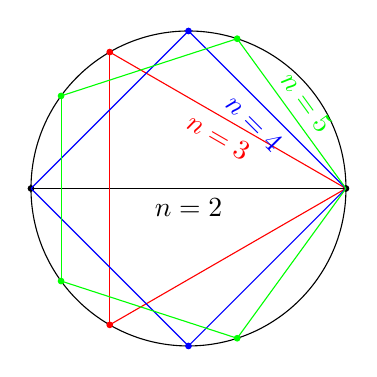
\begin{tikzpicture}
            \path (0: 2) coordinate (P1);
            \path (180: 2) coordinate (P2);

            \path (120: 2) coordinate (Q1);
            \path (240: 2) coordinate (Q2);

            \path (90: 2) coordinate (R1);
            \path (-90: 2) coordinate (R2);

            \path (72: 2) coordinate (S1);
            \path (72*2: 2) coordinate (S2);
            \path (72*3: 2) coordinate (S3);
            \path (72*4: 2) coordinate (S4);

            \draw (0, 0) ellipse (2cm and 2cm);
            \filldraw[black] (P1) circle (1pt);
            \filldraw[black] (P2) circle (1pt);
            \filldraw[red] (Q1) circle (1pt);
            \filldraw[red] (Q2) circle (1pt);
            \filldraw[blue] (R1) circle (1pt);
            \filldraw[blue] (R2) circle (1pt);
            \filldraw[green] (S1) circle (1pt);
            \filldraw[green] (S2) circle (1pt);
            \filldraw[green] (S3) circle (1pt);
            \filldraw[green] (S4) circle (1pt);

            \draw (P1) -- node [anchor=north, sloped]{$n=2$} (P2);

            \draw[red] (P1) -- node [anchor=north, red, sloped]{$n=3$} (Q1) ;
            \draw[red] (Q1) -- (Q2);
            \draw[red] (Q2) -- (P1);

            \draw[blue] (P1) -- node [anchor=north, blue, sloped]{$n=4$} (R1);
            \draw[blue] (P1) -- (R2);
            \draw[blue] (P2) -- (R1);
            \draw[blue] (P2) -- (R2);

            \draw[green] (P1) -- node [anchor=south, green, sloped]{$n=5$} (S1);
            \draw[green] (S1) -- (S2);
            \draw[green] (S2) -- (S3);
            \draw[green] (S3) -- (S4);
            \draw[green] (S4) -- (P1);
        \end{tikzpicture}
    \end{center}


    \begin{th_ex}
        Demuestra que $z^2 + 2z + 4 = 0$ no tiene soluciones en el círculo real.\\

        \textbf{Solución}\\\\
        Basta ver que para que $z$ esté en el círculo real necesitamos que $\vabs{z} \leq 1$. Supongamos que sí, entonces:
        $$
            0 \leq \vabs{z^2+2z} \leq \vabs{z^2} + \vabs{2z} = \vabs{z}^2 + 2\vabs{z} \leq 3
        $$
        Y por tanto, no es posible que al sumar $4$ a $z^2+2z$ resulte $0$.
    \end{th_ex}

    \begin{eg}[Polinomio real]
        Sea $P \in \R[z]$, con $z \in \C$. Entonces:
        \begin{align*}
            P(z):&\ a_0 + a_1z + \cdots + a_{n-1}z^{n-1} = 0\\
            P(\cnj{z}):&\ a_0 + a_1\cnj z + \cdots + a_{n-1}a^{n-1} = 0
        \end{align*}
        y por tanto $P(\cnj z) = P(z)$, entonces $z$ y $\cnj z$ son soluciones del polinomio. Es decir, si $\sdf{a_i}_{\i \in \N} \subset \R$ entonces las raíces son reales o vienen en parejas $z, \cnj z$.
    \end{eg}

    \begin{th_ex}
        Probar que $1 + \cos \frac{2\pi}{n} + \cos \frac{4\pi}{n} + \cdots + \frac{2(n-1)\pi}{n} = 0$.\\

        \textbf{Solución}\\\\
        Notamos que si $w = \cos \frac{2\pi}{n} + i\sin \frac{2\pi}{n} \neq 1$, entonces $w^n = 1$ y por tanto $w$ es una raíz de la unidad.
        \begin{align*}
            w^n &= 1\\
            0 &= 1 - w^n
        \end{align*}
        Podemos factorizar entonces $0 = 1-w^n$:
        $$
            0 = 1-w^n = (1-w)(1+w+\cdots+w^{n-1})
        $$
        Como $(1-w) \neq 0$, entonces $(1+w+\cdots+w^{n-1}) = 0$ y por tanto $\Re(1+w+\cdots+w^{n-1}) = 0$ y vemos que hemos llegado a lo que queremos demostrar:

        $$
            0  =\Re(1+w+\cdots+w^{n-1}) = 1 + \cos \frac{2\pi}{n} + \cos \frac{4\pi}{n} + \cdots + \frac{2(n-1)\pi}{n}
        $$

        De aquí podemos hallar también una igualdad de forma análoga con $\Im(1+w+\cdots+w^{n-1})=0$:
        $$
            \sin \frac{2\pi}{n} + \sin \frac{4\pi}{n} + \cdots + \sin \frac{2(n-1)\pi}{n} = 0
        $$
    \end{th_ex}

    \begin{th_ex}
        Demostrar que $\cos nx$ es un polinomio de $\cos x$ de grado $n$.\\

        \textbf{Solución}\\\\
        $$
            \cos 3x = \Re(\cos x + i\sin x)^3 = \Re(\cos^3 x + 3 \cos^2(x) i \sin(x) - 3 \cos(x)\sin^2(x) - i\sin^3(x))
        $$
        %TODO: Completar
    \end{th_ex}

%%%%%%%%%%%%%%%%%%%%%%%%%%%%%%%%%%%%%%%%%%%%%%%%%%%%%%%%%%%%%%%%%%%%%%%%%% 04/02
\section{Topolg\'ia del plano complejo}

    Podemos definir subconjuntos en el plano con los números complejos.

    \begin{center}
        \begin{tikzpicture}
            \path (30*2: 2) coordinate (W);
            \path (30: 1.2) coordinate (Z);


            \filldraw[black] (W) circle (1pt) node[anchor=west] {$w$};
            \filldraw[black] (Z) circle (1pt) node[anchor=west] {$z$};

            \draw (-2, 0) -- (2, 0);
            \draw (0, -2) -- (0, 2);
            \draw[->] (0, 0) -- (W);
            \draw[->] (0, 0) -- (Z);
            \draw[->] (Z) -- (W);
        \end{tikzpicture}
    \end{center}

    Podemos definir una distancia en $\C$ con el módulo de la siguiente forma:
    $$
        \forall z, w \in \C\ \ \mathrm{dist}(z, w) = \vabs{z - w} = \vabs{\vabs{z-w}}_2
    $$
    y es fácil comprobar que cumple las propiedades de una distancia.\\\\

    \subsection{Bolas y discos en $\C$}
    Ya vimos que podemos definir la circunferencia unidad:\\
    \begin{center}
        \begin{tikzpicture}
            \path (0: 1.5) coordinate (P);


            \draw (0, 0) ellipse (1.5cm and 1.5cm);
            \filldraw[black] (P) circle (1pt) node[anchor=west] {$1$};

            \draw (-2, 0) -- (2, 0);
            \draw (0, -2) -- (0, 2);
        \end{tikzpicture}
    \end{center}
    que se corresponde con el conjunto:
    $$
        \S^1 = \sdf{w \in \C \mid \vabs w = 1} = \sdf{\cos t + i \sin t \mid t \in \left[0, 2\pi\right)}
    $$

    También podemos definir otras bolas o discos en el plano, abiertos o cerrados:\\
    \begin{center}
        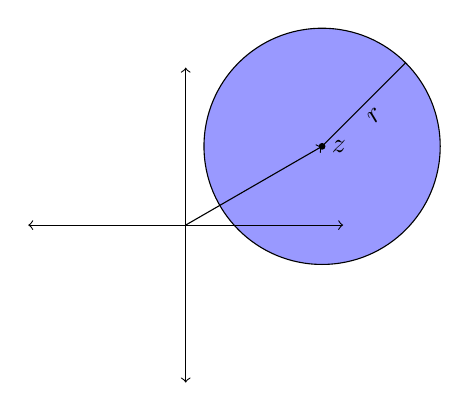
\begin{tikzpicture}
            \path (30: 2) coordinate (Z);
            \filldraw[fill=blue!40!white, draw=black] (Z) circle (1.5cm);
            \filldraw[black] (Z) circle (1pt) node[anchor=west] {$z$};


            \draw (Z) --  node[anchor=north, sloped] {$r$} ++(45:1.5);
            \draw[<->] (-2, 0) -- (2, 0);
            \draw[<->] (0, -2) -- (0, 2);
            \draw[->, thin] (0, 0) -- (Z);
        \end{tikzpicture}
    \end{center}
    Que son los conjuntos definidos por:
    \begin{align*}
        D_r(z) = B_r(z) = B(z, r) &= \sdf{w \in \C \mid \vabs{w - z} < r}\\
        \overline{D_r}(z) = \overline{B_r}(z) = \overline B(z, r) &= \sdf{w \in \C \mid \vabs{w - z} \leq r}\\
        C_r(z) = C(z, r) &= \sdf{w \in \C \mid \vabs{w - z} = r}
    \end{align*}

    \subsection{Rectas en $\C$}
    Las rectas en el plano complejo (a partir de la expresión punto pendiente) se definen como:
    \begin{center}
        \begin{tikzpicture}
            \path (30: 2) coordinate (Z);
            \filldraw[black] (Z) circle (1pt) node[anchor=west] {$z_0$};

            \draw[->] (Z) -- node[anchor=east] {$v$} ++(90:1);
            \draw (1.73205080757, -2) -- (1.73205080757, 2);
            \draw[<->] (-2, 0) -- (2, 0);
            \draw[<->] (0, -2) -- (0, 2);
        \end{tikzpicture}
    \end{center}
    \begin{align*}
        L &= \sdf{z = z_0 + tv \mid t \in \R}\\
          &= \sdf{z-z_0 = tv \mid t \in \R}\\
          &= \sdf{\frac{z-z_0}{v} = t \mid t \in \R} = \sdf{z \in \C \mid \Im\pfrac{z-z_0}{v} = 0}
    \end{align*}

    Es decir, que una recta vertical $S$ que pase por el punto $(1, 0)$ se puede expresar como:
    $$
        S = \sdf{z \in \C \mid \Re(z) = 1} = \sdf{\Re(z) = 1}
    $$

    \subsection{Im\'agenes de conjuntos en $\C$}

    Consideremos ahora:\\
    \fn{$f$}{$\C$}{$\C$}{$z$}{$z^2$}

    Sin duda resulta difícil determinar la imagen de $S$ mediante $f$. Para hallar $f(S)$ necesitamos una descripción algo más detallada de $S$. Comenzamos con:

    $$
        S = \sdf{z=(1, t) \mid t \in \R} = \sdf{z = 1 + ti \mid t \in \R}\\
    $$
    Queremos hallar el conjunto de los cuadrados de los elementos de $S$, entonces:
    $$
        (1+ti)^2 = (1-t^2)+2ti = x + yi
    $$
    de donde obtenemos:
    \begin{align*}
        x(t) &= 1-t^2\\
        y(t) &= 2t\\
        x &= 1-\pfrac{y}{2}^2
    \end{align*}

    Y esto resulta en:
    \begin{center}
        \begin{tikzpicture}
            \draw (1, -3) -- node[anchor=west] {$S$} (1, 3);
            \draw[thick,  domain=-1.5:1.5, samples=40] plot ({1-\x*\x}, {2*\x}) node[anchor=east]{$f(S)$};
            \draw[<->] (-3, 0) -- (3, 0);
            \draw[<->] (0, -3) -- (0, 3);
        \end{tikzpicture}
    \end{center}

    Es fácil ver que para otras rectas verticales cuya parte real es estrictamente positiva, es decir $\sdf{\Re(z)=k>0 \mid k\in \R, \forall z \in \C}$. Sin embargo, si consideramos:
    $$
        L = \sdf{\Re(z) = 0 \mid z\in\C}
    $$
    entonces $f(L)$ es:
    $$
        f(L) = \sdf{(-t^2, 0) \mid t \in \R}
    $$
    es decir, se corresponde con la semirrecta $\R^{-} = (-\infty, 0)$.\\
    \begin{center}
        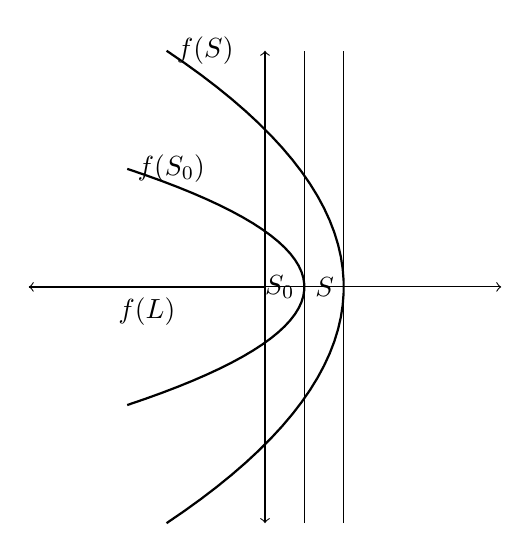
\begin{tikzpicture}
            \draw(0.5, -3) -- node[anchor=east] {$S_0$} (0.5, 3);
            \draw (1, -3) -- node[anchor=east] {$S$} (1, 3);
            \draw[thick,  domain=-1.5:1.5, samples=40] plot ({0.5-\x*\x}, {\x}) node[anchor=west] {$f(S_0)$};
            \draw[thick,  domain=-1.5:1.5, samples=40] plot ({1-\x*\x}, {2*\x}) node[anchor=west] {$f(S)$};
            \draw[thick] (-3, 0) -- node[anchor=north] {$f(L)$} (0, 0);
            \draw[<->] (-3, 0) -- (3, 0);
            \draw[<->] (0, -3) -- (0, 3);
        \end{tikzpicture}
    \end{center}

    Consideremos ahora el semiplano formado por el conjunto de rectas verticales con parte real no negativa $H = \sdf{\Re(z) \geq 0}$. Nos planteamos qué conjunto es $f(H)$. Podemos preguntarnos si $f(H) = \C$, vamos a ver que sí.

    $$
        f(H) = \sdf{z^2 \mid \Re(z) \geq 0} = \sdf{w \in \C \mid \exists z \in H,\ z^2 = w}
    $$
    Es decir, son los cuadrados de los complejos $z \in H$. Si consideramos $w \notin f(H)$, eso querría decir que si $z^2 = w$ entonces $\Re(z) < 0$. Sin embargo, $(-z)^2 = w$ y $\Re(-z) \geq 0$ por tanto, $w \in H$.\\
    Recapitulando, hemos supuesto que existe un $w \in \C$ tal que $w \notin f(H)$ y aún así hemos visto que si pertenece a $\C$. Por tanto $f(H) = \C$

    \begin{th_ex}
        Describe el subconjunto
        $$
            L = \sdf{z \in \C \mid \vabs{z^2-1} < 1}
        $$
        \textbf{Solución}\\\\

%%%%%%%%%%%%%%%%%%%%%%%%%%%%%%%%%%%%%%%%%%%%%%%%%%%%%%%%%%%%%%%%%%%%%%%%%% 05/02
        \begin{align*}
            \sdf{z \in \C \mid \vabs{z^2-1} < 1} &= \sdf{z \in \C \mid \vabs{z^2-1}^2 < 1}\\
            &= \sdf{z \in \C \mid (z^2-1)(\cnj z ^2 - 1) < 1}\\
            &= \sdf{z \in \C \mid \vabs{z}^4 - z^2 - \cnj z ^2 < 0}\\
            &= \sdf{\vabs{z}^4 < z^2 + \cnj z ^2}\\
            &= \sdf{\vabs{z}^4 < \Re(z^2)}
        \end{align*}
        Si $z = \rho (\cos \theta + i \sin \theta)$ tenemos el conjunto:
        $$
            \sdf{\rho^4 < 2 \rho^2 \cos^2 2\theta}
        $$
        Podemos comprobar que $\rho = 0$ no cumple la condición, por tanto, podemos suponer $\rho > 0$ y dividir por $\rho^2$:
        $$
            \sdf{\rho^2 < 2 \cos^2 2\theta}
        $$
        Que son los puntos contenidos en una \textit{lemniscata}.
        \begin{center}
            \begin{tikzpicture}
                \draw[thick,  domain=1:3, samples=100] plot ({sqrt(\x-1)}, {sqrt( sqrt(4*\x-3) -\x)});
                \draw[thick,  domain=1:3, samples=100] plot ({-sqrt(\x-1)}, {sqrt( sqrt(4*\x-3) -\x)});
                \draw[thick,  domain=1:3, samples=100] plot ({sqrt(\x-1)}, {-sqrt( sqrt(4*\x-3) -\x)});
                \draw[thick,  domain=1:3, samples=100] plot ({-sqrt(\x-1)}, {-sqrt( sqrt(4*\x-3) -\x)});
                \draw[<->] (-3, 0) -- (3, 0);
                \draw[<->] (0, -2) -- (0, 2);
            \end{tikzpicture}
        \end{center}
    \end{th_ex}

    \begin{th_ex}
        Describe el subconjunto
        $$
            H = \sdf{z \in \C \mid \Im\pfrac{z-z_0}{v} > 0}
        $$
        con $z_0, v \in  \C$\\

        \textbf{Solución}\\\\

        Ya hemos visto que la expresión de una recta con vector director $v$ y que pasa por el punto $z_0$ tiene la expresión:
        $$
            \sdf{z \in \C \mid \Im\pfrac{z-z_0}{v} = 0}
        $$
        Por lo que cabría esperar que el conjunto que buscamos tiene alguna relación con la recta, y probablemente sea uno de los dos semiplanos definidos por la misma.\\
        Consideremos $w = \frac{z-z_0}{v} = a + bi$. Entonces podemos reescribir el conjunto $H$:
        $$
            H = \sdf{z \mid w = \frac{z-z_0}{v} = a + bi,\ b>0}
        $$
        Desarrollamos la igualdad del conjunto:
        \begin{align*}
            z - z_0 &= v (a + bi)\\
            z &= z_0 + v(a + bi)\\
                &= z_0 + av + i\cdot bv
        \end{align*}
        Es decir, que los $z$ de $H$ son los puntos a los que llegamos de desplazarnos una cantidad en la recta $z_0 + av$ (recordemos que $v$ es vector director de la recta) y además, nos movemos en sentido positivo ($b>0$) en la dirección $i\cdot v$, es decir, el giro de $\sfrac{\pi}{2}$ en sentido positivo de $v$.\\

        De esta forma, es claro ver que $H \subseteq \Pi$ donde $\Pi$ es el semiplano \textit{a la izquierda} del vector director $v$. Faltaría demostrar que $\Pi \subseteq H$.
        \begin{center}
            \begin{tikzpicture}
                \path (1.5, 1) coordinate (X);
                \path (2, 2) coordinate (V);
                \path (X) + (60+90: 1) coordinate (iV);
                \path (1.25, 0.5) coordinate (Y);
                \path (Y) + (60+90: 1.5) coordinate (W);
                \draw[<->] (-3, 0) -- (3, 0);
                \draw[<->] (0,-2) -- (0, 2);
                \draw[thick,  domain=0:2, samples=100] plot ({\x}, {2*(\x-1)});
                \draw[dashed, ->] (X) -- (iV) node[anchor=south] {$iv$};
                \draw[red, ->] (X) -- (V) node[anchor=south] {$v$};
                \draw[->] (X) -- node[anchor=north, sloped] {$av$} (Y);
                \draw[->] (Y) -- node[anchor=north, sloped] {$ibv$} (W);
                \filldraw[black] (X) circle (1pt) node[anchor=west] {$z_0$};
                \filldraw[blue] (Y) circle (1pt) node[anchor=north] {$z_0 + av$};
                \filldraw[black] (W) circle (1pt) node[anchor=north] {$z$};
            \end{tikzpicture}
        \end{center}
    \end{th_ex}

\section{Esfera de Riemann}
    En ocasiones nos enfrentaremos a ecuaciones que no tienen solución en $\C$, como:
    $$
        w = \frac{1}{z}
    $$
    Para solucionar esto, vamos a \textbf{completar} $\C$, y vamos a añadir un punto a $\C$ que es la solución a la ecuación superior. Llamaremos a este punto $\infty$ y denominamos extensión de $\bar \C = \C \cup \sdf{\infty}$.\\\\
    El plano complejo extendido se puede visualizar gracias a la proyección estereográfica de la esfera sobre el plano.
    \begin{center}
        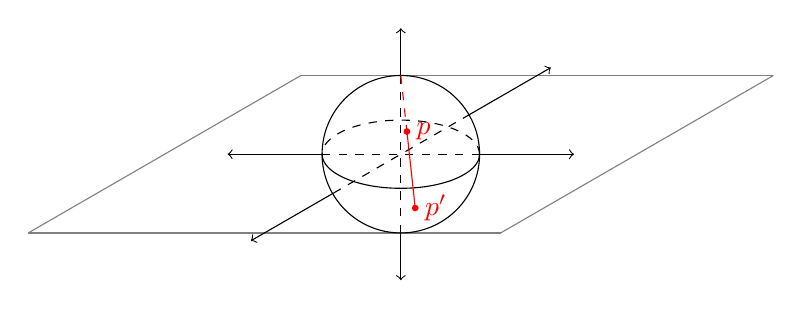
\begin{tikzpicture}[scale=1]
            %Radius
            \def\R{1};
            \path (0, 0) coordinate (O);
            \path (0, 1) coordinate (N);
            % Plane corners
            \path (1.26794919, -1) coordinate (P1);
            \path (-4.73205081, -1) coordinate (P2);
            \path (-1.26794919, 1) coordinate (P3);
            \path (4.73205081, 1) coordinate (P4);

            \path (-0.854161, -0.49315) coordinate (P);

            % Point and projection
            \path (0.07735027, 0.28867513) coordinate (S);
            \path (0.1830127, -0.6830127) coordinate (S');
            % Plane
            \draw[thin, gray] (P1) -- (P2);
            \draw[thin, gray] (P2) -- (P3);
            \draw[thin, gray] (P3) -- (P4);
            \draw[thin, gray] (P4) -- (P1);
            % Axes
            \draw[->] (0, \R) -- (0, \R+0.6);
            \draw[->] (0, -\R) -- (0, -\R-0.6);
            \draw[<-] (-\R-1.2, 0) -- (-\R, 0);
            \draw[->] (\R, 0) -- (\R+1.2, 0);
            \draw[dashed] (-\R, 0) -- (\R, 0);
            \draw[dashed] (0, -\R) -- (0, \R);
            \draw[dashed] (P) -- (30: \R);
            \draw[->] (P) -- (210: \R+1.2);
            \draw[->] (30:\R) -- (30:\R+1.2);

            % Sphere
            \draw (O) circle (\R);
            \draw (-\R, 0) arc (180:360:\R cm and 0.43301270189221935cm);
            \draw[dashed] (\R, 0) arc (0:180:\R cm and 0.43301270189221935cm);

            % Point and projection
            \draw[dashed, red] (0, \R) -- (S);
            \draw[red] (S) -- (S');
            \filldraw[red] (S) circle (1pt) node[anchor=west]{$p$};
            \filldraw[red] (S') circle (1pt) node[anchor=west]{$p'$};
        \end{tikzpicture}
    \end{center}
    Vemos que la forma de relacionar $\C$ y $\S^2$ (la esfera unidad) es proyectar cada punto de la superficie de la esfera desde el punto $(0, 0, 1)$ hacia el plano, es decir, si $p = (x, y, z)$, su proyección $p'$ es la intersección del plano con la recta que une $p$ y $(0, 0, 1)$.\\

    \begin{obs}
        \begin{center}
            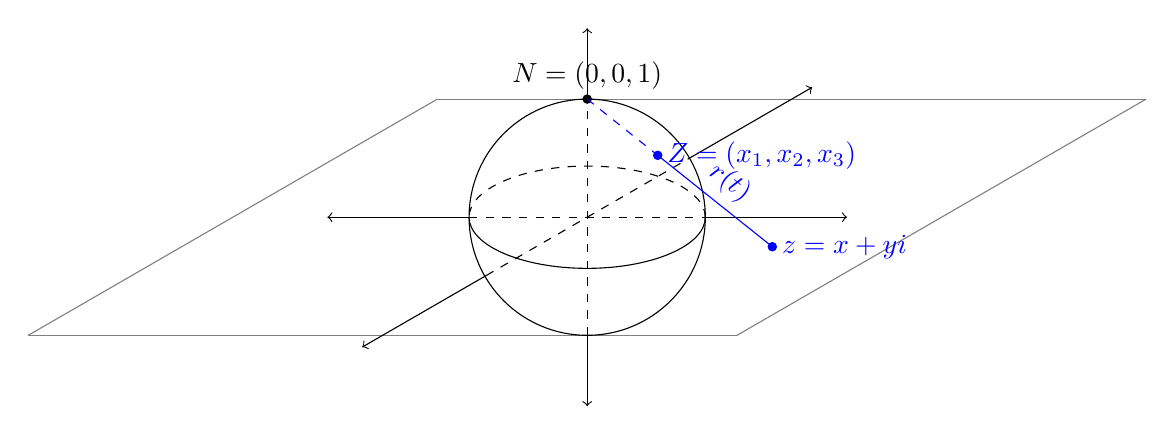
\begin{tikzpicture}[scale=1.5]
                %Radius
                \def\R{1};
                \path (0, 0) coordinate (O);
                \path (0, 1) coordinate (N);
                % Plane corners
                \path (1.26794919, -1) coordinate (P1);
                \path (-4.73205081, -1) coordinate (P2);
                \path (-1.26794919, 1) coordinate (P3);
                \path (4.73205081, 1) coordinate (P4);

                \path (-0.854161, -0.49315) coordinate (P);

                % Point and projection
                \path (0.59694754, 0.52380952) coordinate (S);
                \path (1.5669873, -0.25) coordinate (S');
                % Plane
                \draw[thin, gray] (P1) -- (P2);
                \draw[thin, gray] (P2) -- (P3);
                \draw[thin, gray] (P3) -- (P4);
                \draw[thin, gray] (P4) -- (P1);
                % Axes
                \draw[->] (0, \R) -- (0, \R+0.6);
                \draw[->] (0, -\R) -- (0, -\R-0.6);
                \draw[<-] (-\R-1.2, 0) -- (-\R, 0);
                \draw[->] (\R, 0) -- (\R+1.2, 0);
                \draw[dashed] (-\R, 0) -- (\R, 0);
                \draw[dashed] (0, -\R) -- (0, \R);
                \draw[dashed] (P) -- (30: \R);
                \draw[->] (P) -- (210: \R+1.2);
                \draw[->] (30:\R) -- (30:\R+1.2);

                % Sphere
                \draw (O) circle (\R);
                \draw (-\R, 0) arc (180:360:\R cm and 0.43301270189221935cm);
                \draw[dashed] (\R, 0) arc (0:180:\R cm and 0.43301270189221935cm);
                \filldraw[black] (N) circle (1pt) node[anchor=south]{$N = (0, 0, 1)$};
                % Point and projection
                \draw[dashed, blue] (0, \R) -- (S);
                \draw[blue] (S) -- node[anchor=south, sloped]{$r(t)$}(S');
                \filldraw[blue] (S) circle (1pt) node[anchor=west]{$Z = (x_1, x_2, x_3)$};
                \filldraw[blue] (S') circle (1pt) node[anchor=west]{$z = x+ yi$};
            \end{tikzpicture}
        \end{center}
        Si queremos encontrar $Z$ en función de $z$, sea $r(t)$ la recta que une $N$ y $z$, entonces $r(t)$ interseca a la esfera en $Z$. La ecuación de esta recta es:
        \begin{align*}
            r &= \sdf{tN + (1-t)Z \mid t \in \R}\\
            &= \sdf{t(0, 0, 1) + (1-t)(x, y, 0) \mid t \in \R}\\
            &= \sdf{((1-t)x, (1-t)y, t) \mid t \in \R}
        \end{align*}
        y además, sea $r(t)$ el punto de la recta $r$ para un valor de $t$:
        \begin{align*}
            r(t) \in S &\iff  (1-t)^2x^2+(1-t)^2y^2+t^2 = 1\\
                       &\iff (1-t)^2\vabs{z}^2 + t^2 = 1
        \end{align*}
        Podemos desarrollar esta última igualdad para hallar las coordenadas de $Z$:
        \begin{align*}
            (1-t)^2 \vabs{z}^2 + t^2 &= 1\\
            (1-t)^2 \vabs{z}^2 &= 1 - t^2\\
            (1-t)(1-t)\vabs{z}^2 &= (1-t)(1+t)\\
            (1-t)\vabs{z}^2 &= 1+t\\
            \vabs{z}^2 - 1 &= t(1+\vabs{z}^2)\\
            t &= \frac{\vabs{z}^2 -1}{\vabs{z}^2+1}
        \end{align*}
        Y hallamos:
        \begin{align*}
            Z &= \px{\frac{2x}{\vabs{z}^2+1}, \frac{2y}{\vabs{z}^2+1}, \frac{\vabs{z}^2-1}{\vabs{z}^2+1}}\\
            &= \px{\frac{z+\cnj z}{\vabs{z}^2+1}, \frac{-i(z-\cnj z)}{\vabs{z}^2+1}, \frac{\vabs{z}^2-1}{\vabs{z}^2+1}}
        \end{align*}

        Supongamos ahora conocido un punto $Z = (x_1, x_2, x_3) \in \S^2\setminus\sdf{(0, 0, 1)}$. ¿Cómo encontramos $z\in\C$ su proyección en el plano complejo?

        Como hemos visto, es el punto de corte entre el plano y la recta que une $Z$ y $N = (0, 0, 1)$, entonces:
        \begin{align*}
            (x_1, x_2, x_3) &= Z = t (0, 0, 1) + (1-t)(x, y, 0)\\
            x_1 &= (1-t) x\\
            x_2 &= (1-t) y\\
            x_3 &= t
        \end{align*}

        Basta resolver este sistema con lo que hallamos:
        \begin{align*}
            x = \frac{x_1}{1-t} = \frac{x_1}{1-x_3}\\
            y = \frac{x_2}{1-t} = \frac{x_2}{1-x_3}
        \end{align*}
    \end{obs}

%%%%%%%%%%%%%%%%%%%%%%%%%%%%%%%%%%%%%%%%%%%%%%%%%%%%%%%%%%%%%%%%%%%%%%%%%% 06/02
    \begin{ex}[H1.2]\label{ex:h1.2}
        Calcule los valores:
        \begin{enumerate}[a)]
            \item $\vabs{(2-i)(1+i)^4}$
            \item $\vabs{\frac{1+i\sqrt 3}{4-3i}}$
            \item $\sum_{k=1}^{2020} i^k$
        \end{enumerate}
        \textbf{Solución}\\\\
        \begin{enumerate}[a)]
            \item
            \item
            \item
            Notamos que $i + i^2 + i^3 + i^4 = i -1 +i +1 = 0$ y por tanto como $2020$ es múltiplo de $4$
            $$
                \sum_{k=1}^{2020} i^k = \sum_{j=1}^{505} i^{4j} + i^{4j+1} + i^{4j+2} + i^{4j+3} = \sum_{j=1}^{505} 0 = 0
            $$
        \end{enumerate}
    \end{ex}

    \begin{ex}[H1.3]
        Compruebe la identidad $\vabs{1+z\cnj w}^2 + \vabs{z-w^2} = (1+\vabs{z}^2)(1+\vabs{w}^2)$ para todo $z, w \in \C$.\\

        \textbf{Solución}\\\\
        \begin{align*}
            \vabs{1+z\cnj w}^2 + \vabs{z-w^2} &= (1+z\cnj w)(1+\cnj z w) + (z-w)(\cnj z - \cnj w)\\
            &= 1+ \cancel{z\cnj{w}} + \cancel{\cnj{z} w} + z\cnj{z}\cnj{w}w + z\cnj{z} - \cancel{z\cnj{w}} - \cancel{w\cnj{z}} + w\cnj{w} \\
            &= 1 + \vabs{z}^2 + \vabs{w}^2 + \cnj{z}^2\vabs{w}^2\\
            &= (1+\vabs{z}^2)(1+\vabs{w}^2)
        \end{align*}
    \end{ex}

    \begin{ex}[H1.4]
        Demuestre la \textit{identidad de Lagrange}: si $z_1, z_2, \ldots, z_n$ y $w_1, w_2, \ldots, w_n$ son números complejos, entonces
        $$
            \px{\sum_{j=1}^{n} \vabs{z_j}^2} \px{\sum_{j=1}^n \vabs{w_j}^2} - \vabs{\sum_{j=1}^n z_jw_j}^2 = \sum_{1\leq i<j\leq n} \vabs{z_i \cnj{w_j} - z_j \cnj{w_i}}^2
        $$
        \textbf{Solución}\\\\
        Vamos a comenzar escribiendo la igualdad de otra forma y desarrollando $S_1$
        $$
        \underbracket{\px{\sum_{j=1}^{n} \vabs{z_j}^2} \px{\sum_{j=1}^n \vabs{w_j}^2}}_{S_1} = \underbracket{\vabs{\sum_{j=1}^n z_jw_j}^2 + \sum_{1\leq i<j\leq n} \vabs{z_i \cnj{w_j} - z_j \cnj{w_i}}^2}_{S_2}
        $$
        \begin{align*}
            \px{\sum_{j=1}^{n} \vabs{z_j}^2} \px{\sum_{j=1}^n \vabs{w_j}^2} &= \sum_{i=j}^n \vabs{z_iw_j}^2 + \sum_{i\neq j}^n \vabs{z_iw_j}^2\\
            &= \sum_{i=1}^n \vabs{z_iw_i}^2 + \sum_{1 \leq i < j \leq n} \px{\vabs{z_iw_j}^2 + \vabs{z_jw_i}^2}\\
            &= \underbracket{\sum_{i=1}^n \vabs{z_iw_i}^2}_{P_1}+ \underbracket{\sum_{1 \leq i < j \leq n} \px{\vabs{z_iw_j}^2 + \vabs{z_jw_i}^2}}_{P_2}\\
        \end{align*}
        Entonces tenemos que ver si $S_2$ es igual a lo anterior. Vamos a desarrollar un término de $S_2$
        \begin{align*}
            \vabs{\sum_{j=1}^n z_jw_j}^2 &= (z_1w_1 + \ldots + z_nw_n)(\cnj{z_1}\cnj{w_1} + \ldots \cnj{z_n}\cnj{w_n})\\
            &= \sum_{1 \leq i, j \leq n} z_iw_i\cnj{z_j}\cnj{w_j} = \sum_i^n \vabs{z_i}^2 \vabs{w_i}^2 + \sum_{1 \leq i < j \leq n} z_i\cnj{z_j}w_i\cnj{w_j} + z_j\cnj{z_i} + w_j\cnj{w_i}\\
            &= P_1 + \underbracket{\sum_{1 \leq i < j \leq n} z_i\cnj{z_j}w_i\cnj{w_j} + z_j\cnj{z_i} + w_j\cnj{w_i}}_{P_3}
        \end{align*}
        Por tanto podemos cancelar $P_1$ y entonces tenemos que demostrar:
        $$
            P_2 = P_3 + \underbracket{\sum_{1 \leq i < j \leq n} \vabs{z_i\cnj{w_j} - z_j\cnj{w_i}}^2}_{P_4}
        $$
        Y si desarrollamos $P_4$ obtenemos
        $$
            P_4 = \sum_{1 \leq i < j \leq n} (z_i\cnj{w_j} - z_j\cnj{w_i}) (\cnj{z_i} w_j  - \cnj{z_j} w_i )
        $$
        Que es $P_2 - P_3$ y hemos terminado.
    \end{ex}

    \begin{ex}[H1.5]
        Demuestre las siguientes afirmaciones:
        \begin{enumerate}[a)]
            \item Si $a, b \in \C$ y $z \in \C\setminus\sdf{-\cnj{\pfrac{a}{b}}}$ con $\vabs{z} = 1$, entonces se cumple $\vabs{\frac{az+b}{\cnj b z + \cnj a}} = 1$
            \item Si $\vabs{a} < 1$, entonces $\vabs{z} < 1$ es equivalente a $\vabs{\frac{z-a}{1-\cnj a z}} < 1$
        \end{enumerate}
        \textbf{Solución}\\\\
        \begin{enumerate}[a)]
            \item
                \begin{align*}
                    \vabs{az+b} = \vabs{\cnj b z + \cnj a} &\iff \vabs{az+b}^2 = \vabs{\cnj b z + \cnj a}^2\\
                    &\iff (az + b)(\cnj a \cnj z + \cnj b) = (\cnj b z + \cnj a)(b \cnj z + a)
                \end{align*}
                Entonces basta demostrar
                \begin{align*}
                    (az + b)(\cnj a \cnj z + \cnj b) &= (\cnj b z + \cnj a)(b \cnj z + a)\\
                     \vabs{a}^2 \vabs{z}^2 + \vabs{b}^2 + \cancel{a\cnj b z + b \cnj a \cnj z} &= \vabs{b}^2 \vabs{z}^2 + \vabs{a}^2 + \cancel{a\cnj b z + b \cnj a \cnj z}
                \end{align*}
                Y como $\vabs{z} = 1$ hemos terminado.
        \end{enumerate}
    \end{ex}


    Con esta proyección, todo $\C$ queda cubierto por la proyección de $\S^2\setminus\sdf{(0, 0, 1)}$. Por tanto, existe un $F: \C \to \S^2\setminus\sdf{(0, 0, 1)}$ homeomorfismo.\\
    Diremos que $\infty \in \C$ es la proyección del punto $(0, 0, 1)$. Llamaremos $\overline{\C} = \C \cup \sdf{\infty}$ y lo leeremos como $\C$ extendido y ahora tenemos un homeomorfismo $f: \overline{\C} \to \S^2$.\\

    Nos gustaría además poder definir una distancia en $\cnj \C$ que induzca en $\C$ la topología usual. Recordamos que sea $Z \in \S^2$ un punto de la esfera unidad y $z$ su proyección en el plano complejo entonces llamamos $f(z)$ a
    $$
        f(z) = Z = \px{\frac{z+\cnj z}{\vabs{z}^2+1}, \frac{-i(z-\cnj z)}{\vabs{z}^2+1}, \frac{\vabs{z}^2-1}{\vabs{z}^2+1}}
    $$
    Vamos a definir la distancia entre $z, z' \in \cnj \C$ como:
    $$
        d(z, z') = \vabs{\vabs{f(z) - f(z')}}_2
    $$
    es decir, es la distancia en $R^3$ entre la proyección sobre la esfera unidad del plano complejo extendido.

    \begin{th_ex}
        Encontrar la expresión de $d(z, z')$ y $d(z, \infty)$.
    \end{th_ex}


\section{Sucesiones en $\C$}
    Cuando tengamos una sucesión de complejos $\sdf{z_n}$ diremos que
    $$
        \sdf{z_n} \to z \iff \sdf{\vabs{z_n - z}} \to 0
    $$
    Es decir, que para cada $\varepsilon > 0$, $\exists n_0 \in \N$ tal que $Z_n \in D(z, \varepsilon) \forall n \geq n_0$\\

    \begin{center}
        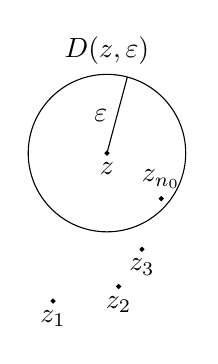
\begin{tikzpicture}
            \path (0, 0) coordinate (Z);
            \path (250:2) coordinate (Z1);
            \path (275:1.7) coordinate (Z2);
            \path (290:1.3) coordinate (Z3);
            \path (320: 0.9) coordinate (Z0);

            \draw (Z) circle (1cm);
            \draw (0, 1)  node[anchor=south] {$D(z, \varepsilon)$};
            \filldraw[black] (Z) circle (0.7pt) node[anchor=north] {$z$};
            \filldraw[black] (Z1) circle (0.7pt) node[anchor=north] {$z_1$};
            \filldraw[black] (Z2) circle (0.7pt) node[anchor=north] {$z_2$};
            \filldraw[black] (Z3) circle (0.7pt) node[anchor=north] {$z_3$};
            \filldraw[black] (Z0) circle (0.7pt) node[anchor=south] {$z_{n_0}$};
            \draw (Z) -- node[anchor=east] {$\varepsilon$} (75:1);
        \end{tikzpicture}
    \end{center}
    Además, utilizando las propiedades de las normas $p$, podemos obtener el siguiente resultado.
    \begin{pro}[L\'imite de una sucesión compleja]
        Sea $\sdf{z_n}$ una sucesión compleja
        $$\sdf{z_n} \to_{n\to\infty} z \iff \sdf{\Re(z_n)}\to \Re(z) \text{ y } \sdf{\Im(z_n)}\to \Im(z)$$
    \end{pro}
    \begin{proof}
        Se deja al lector.
    \end{proof}

    \begin{pro}[Condici\'on necesaria y suficiente para el l\'imite de una sucesi\'on compleja]
        Sea $\sdf{z_n}$ una sucesión compleja
        $$\sdf{z_n} \to_{n\to\infty} z \iff \vabs{z_n - z} \to 0$$
    \end{pro}
    \begin{proof}
        Se deja al lector.
    \end{proof}


    \begin{th_ex}
        Demostrar que $\sdf{z^n}$ con $z$ en la circunferencia solo converge si $z = 1$.
    \end{th_ex}

    \begin{pro}[Convergencia absoluta de una sucesi\'on]
        Sea $\sdf{z_n}$ una sucesión compleja
        $$
            \sdf{z_n} \to z \implies \sdf{\vabs{z_n}} \to z
        $$
    \end{pro}
    \begin{proof}
        Si $\sdf{z_n} \to z \implies \vabs{z_n - z} \to 0$. Además sabemos que:
        $$
            0 \leq \vabs{\vabs{z_n} - \vabs{z}} \leq \vabs{z_n - z}
        $$
        Y tomando límites en cada término de la desigualdad, vemos que:
        $$
            0 \leq \lim_{n \to \infty} \vabs{\vabs{z_n} - \vabs{z}} \leq 0
        $$
        Y por tanto por el lema del Sandwich
        $$
        \lim_{n \to \infty} \vabs{\vabs{z_n} - \vabs{z}} = 0 \implies \sdf{\vabs{z_n}} \to \vabs{z}
        $$
    \end{proof}

    \begin{eg}[Límite de una sucesión]
        Sea la sucesión $\sdf{z_n} = \sdf{\frac{n}{n+i}}$, no es descabellado pensar que el límite es $1$, veámoslo:
        $$
            \vabs{\frac{n}{n+i} - 1} = \vabs{\frac{n}{n+i} - \frac{n+i}{n+i}} = \vabs{\frac{-i}{n+i}} = \frac{1}{\vabs{n+i}} = \frac{1}{\sqrt{n^2-1}}
        $$
        y efectivamente $\frac{1}{\sqrt{n^2-1}} \to_{n\to\infty} 0 \implies \sdf{z_n} \to 1$
    \end{eg}

    \begin{obs}[Convergencia de una serie]
        Diremos que $$\sum_{n=1}^{\infty}  z_n = z \iff \sdf{\sum_{n=1}^{m} z_n} \to_{m\to\infty} z$$
    \end{obs}

    \begin{pro}[Convergencia y sucesión de Cauchy]
        Sea $\sdf{z_n}$ una sucesión en $\C$
        $$
            \sdf{z_n} \text{ es convergente } \iff \sdf{z_n} \text{ es de Cauchy }
        $$
    \end{pro}
    \begin{proof}
        Se deja al lector.
    \end{proof}

    \begin{pro}[Resultados varios de convergencia]$ $
        \begin{enumerate}[1)]
            \item Sean $S_1$, $S_2$ dos series convergentes, entonces $S_1 + S_2$ es convergente.
            \item Si $\sum z_n$ es convergente, entonces $\sdf{z_n} \to_{n\to \infty} 0$.
            \item Si $\sum \vabs{z_n}$ es convergente, entonces $\sum \vabs{z_n}$ es convergente.
            \item $A$ compacto $\iff$ $A$ es cerrado y acotado (en $\C$).
        \end{enumerate}
    \end{pro}
    \begin{proof}
        Se deja al lector.
    \end{proof}

    \begin{eg}[Convergencia de series]$ $
        \begin{enumerate}[a)]
            \item $\sum_{k=1}^{\infty} \frac{i^k}{k^2+i}$,
            $$
                \vabs{\frac{i^k}{k^2+1}} = \vabs{\frac{1}{k^2+i}} = \frac{1}{\vabs{k^2+i}} = \frac{1}{k^4+1} \leq \frac{1}{k^2}
            $$
            y entonces
            $$
                \sum \frac{1}{k^2} \text{ converge } \implies \sum \vabs{\frac{i^k}{k^2+i}} \text{ converge } \implies \sum_{k=1}^{\infty} \frac{i^k}{k^2+i} \text{ converge }
            $$
            \item $\sum_{k=1}^{\infty} \frac{1}{k+i} = \sum_{k=1}^{\infty} \frac{k-i}{k^2+1}$.\\

            La parte real $\sum \frac{k}{k^2+1}$ es comparable a $\sum \frac{1}{k}$ que no es convergente, por tanto como su parte real no converge la serie tampoco lo hace.
        \end{enumerate}
    \end{eg}

\section{Funciones complejas}

    En secciones anteriores ya hemos vistos los efectos de la función $f(x) = x^2$ a algunos conjuntos definidos en $\C$. No todas las funciones van a ser objeto de estudio de la asignatura. Comenzamos restringiéndonos al estudio de funciones continuas.

    \subsection{Funciones continuas complejas}
    \begin{dfn}[Funci\'on continua]
        Sea $z_0 \in \C$ arbitrario y $\mathcal{U}(z_0)$ un entorno de $z_0$. Sea $f: \mathcal{U}(z_0) \to \C$ una función compleja, diremos que $f$ es $\mathbf{continua}$ en $z_0$ si $\sdf{f(z_n)} \to f(z_0)$ para toda sucesión $\sdf{z_n} \to z_0$.\\

        Si $f$ es continua en todo su dominio, se dice simplemente que es continua.
    \end{dfn}

    En ocasiones podremos analizar una función $f$ compleja como una función hacia $\R \times \R$, es decir\\

    \fn{$f$}{$\mathcal D \subseteq \C$}{$\R \times \R$}{$z$}{$(u(z), v(z)) \equiv u(z) + i v(z)$}

    Donde $u, v: \C \to \R$ son funciones escalares. En este caso podemos afirmar el resultado siguiente.
    \begin{pro}
        Sea $f$ una función compleja. Sean $u, v$ funciones escalares tales que $f(z) = (u(z), v(z))$, entonces:
        $$
            f \text{ es continua } \iff u, v \text{ son continuas }
        $$
    \end{pro}

    \begin{ex}[H2.10]\label{ex:2.10}Demuestre que\\
        \begin{enumerate}[a)]
            \item $\sin(3x) = 3\sin(x) - 4\sin^3(x)$ para todo $x \in \R$.
            \item $\forall \theta \in \px{\frac{-\pi}{2}, \frac{\pi}{2}}$ se cumple
            $$
                \pfrac{1+i\tan \theta}{1 - i \tan \theta}^n = \frac{1 + i\tan \theta}{1 - i \tan \theta}
            $$
        \end{enumerate}
        \textbf{Solución}\\\\
        \begin{enumerate}
            \item
            \begin{align*}
                z &= \cos(x) + i \sin(x)\\
                z^3 &= (\cos(x) + i\sin(x))^3 \implies \sin(3x) = \Im(z^3)\\
                    &= \cos^3(x) + 3\cos^2(x) i \sin(x) - 3 \cos(x)\sin^2(x) - i \sin^3(x)\\
                    &= \cos^3(x)-3\cos(x)+(3\cos^2(x)\sin( x) - \sin^3(x))i
            \end{align*}
            Y entonces $\Im(z^3) = 3(1 - \sin^2(x))\sin(x) - \sin^3(x) = 3 \sin(x) - 4 \sin^3(x)$ y como $\Im(z^3) = \sin(3x)$ hemos terminado.
            \item Comenzamos observando que el denominador siempre tiene parte real $1$, por lo que la división está bien definida. Ahora multiplicamos todo por $\frac{\cos^n \theta}{\cos^n \theta}$.
            \begin{align*}
                \frac{\cos^n \theta}{\cos^n \theta} \frac{1 + i\pfrac{\sin \theta}{\cos \theta}}{1 - i\pfrac{\sin \theta}{\cos \theta}} = \frac{(\cos \theta + i \sin \theta)^n}{(\cos \theta - i \sin \theta)^n} = \frac{(\cos n\theta + i \sin n\theta)}{(\cos n\theta + i \sin n\theta)} = \frac{1 + i\tan \theta}{1 - i \tan \theta}
            \end{align*}
        \end{enumerate}
    \end{ex}

    \begin{obs}$ $
        \begin{enumerate}[a)]
            \item $\sin(nx)$ no es un polinomio de $\sin(x)$.
            \item En el ejercicio \ref{ex:2.10}(b), hemos usado \hyperref[eg:DeMoivre]{la fórmula de De Moivre} pero con $(\cos \theta \mbf{-} i \sin \theta)$ en lugar de $(\cos \theta + i \sin \theta)$, sin embargo, basta observar que $(\cos \theta - i \sin \theta) = \cnj z$ y como podemos intercambiar conjugados y potencias
            $$(\cos \theta \mbf{-} i \sin \theta)^n = (\cnj z)^n = \cnj{z^n} = \cnj{(\cos \theta + i \sin \theta)^n} = \cnj{\cos n\theta + i \sin n\theta} = \cos n\theta - i \sin n\theta$$
        \end{enumerate}
    \end{obs}

    \begin{ex}[H2.15]\label{eg:2.15}
        Resuelva en $\C$ la ecuación: $\cnj z = z^{n-1}$, $n\in \N$.\\

        \textbf{Solución}\\\\
        \begin{enumerate}[1)]
            \item $0$ es solución.
            \item Si $z \neq 0$, entonces multiplicando todo por $z$ entonces $\cnj z \cdot z = z^n$, y por tanto $\vabs{z}^2 = z^n$ y necesariamente $z^n$ es un número real. Así que podemos escribir:
            $$
                \vabs{z}^2 = \vabs{ \vabs{z}^2 } = \vabs{z^n} = \vabs{z}^n
            $$
            Si $n > 2$, entonces dividiendo por $\vabs{z}^2$ obtenemos $1 = \vabs{z}^{n-2} \implies \vabs{z} = 1$. Retomando nuestra igualdad anterior, sustituyendo $\vabs{z}=1$:
            $$
                1 = \cnj z \cdot z = z^n
            $$
            es decir, $z$ es una raíz $n$-ésima de la unidad.\\\\
            Si $n=2$, entonces estamos en el caso $\cnj z = z$, es decir, $z \in \R$ y por tanto cualquier $x \in \R$ es solución de la ecuación.\\\\
            Finalmente, si $n = 0$, tenemos la ecuación $\cnj z = z^{1-1} = z^0 = 1$, es decir, $\cnj z = 1 \implies z = 1$.
        \end{enumerate}
    \end{ex}
% \section{L\'imites y continuidad}
